%%%%%%%%%%%%%%%%%%%%%%%%%%%%%%%%%%%%%%%%%
% University/School Laboratory Report
% LaTeX Template
% Version 3.1 (25/3/14)
%
% This template has been downloaded from:
% http://www.LaTeXTemplates.com
%
% Original author:
% Linux and Unix Users Group at Virginia Tech Wiki 
% (https://vtluug.org/wiki/Example_LaTeX_chem_lab_report)
%
% License:
% CC BY-NC-SA 3.0 (http://creativecommons.org/licenses/by-nc-sa/3.0/)
%
%%%%%%%%%%%%%%%%%%%%%%%%%%%%%%%%%%%%%%%%%

%----------------------------------------------------------------------------------------
%	PACKAGES AND DOCUMENT CONFIGURATIONS
%----------------------------------------------------------------------------------------

\documentclass{article}
\usepackage{graphicx}
\usepackage[utf8]{inputenc}
\usepackage{amsmath} % Required for some math elements 
\usepackage[italian]{babel}
\setlength\parindent{0pt} % Removes all indentation from paragraphs
\usepackage[style=authortitle-comp,	backend=biber]{biblatex}
\renewcommand{\labelenumi}{\alph{enumi}.} % Make numbering in the enumerate environment by letter rather than number (e.g. section 6)

%\usepackage{times} % Uncomment to use the Times New Roman font

%----------------------------------------------------------------------------------------
%	DOCUMENT INFORMATION
%----------------------------------------------------------------------------------------

\title{Classificazione di Tweet a tema politico} % Title

\date{\today} % Date for the report

\author{Simone \textsc{Robutti}} % Author name
\addbibresource{main.bib}
\begin{document}

\maketitle % Insert the title, author and date
\begin{center}
\textsc{Matricola: 823523}

\end{center} 

% If you wish to include an abstract, uncomment the lines below
% \begin{abstract}
% Abstract text
% \end{abstract}

%----------------------------------------------------------------------------------------
%	SECTION 1
%----------------------------------------------------------------------------------------
\tableofcontents


\section{Introduzione ed Obiettivi}
L'esperimento si propone di generare un classificatore in grado di discernere l'orientamento politico di un utente Twitter basandosi sul contenuto dei suoi Tweet.

Il lavoro si sviluppa partendo dal lavoro e dalle considerazioni di \cite{sides}. La differenza fondamentale con questo lavoro è la natura dei testi classificati: non Tweet ma post di un forum di politica, quindi più lunghi e argomentati e con uno spettro sintattico e semantico più ampio.

Altri lavori simili presi in considerazione sono \cite{pennacchiotti} e \cite{durant} che però per complessità e obiettivi sono lontani da quanto realizzato.


\section{Metodologia e approccio}

Per rappresentare i tweet nello spazio delle features si è scelto di usare un modello bag of words associando ad ogni parola presente o assente un valore binario. Utilizzare il numero di occorrenze di una parola all'interno del tweet è un approccio valutato da \cite{sides} e sconsigliato perché dava risultati leggermente peggiori.

Lo spazio delle etichette è stato poi suddiviso in 4 classi: "Sinistra","Destra", "Centro" e "Populisti". Una divisione in due sole classi ("Sinistra" e "Destra" o "Conservatori" e "Progressisti") mal si prestava a rappresentare lo scenario politico e mediatico italiano odierno. 

Essendo l'informazione presente nel singolo tweet insufficiente, si è scelto per raggruppare i tweet in gruppi di dimensione fissata e determinata empiricamente come documentato in seguito. Inoltre il raggruppamento nel training set non viene fatto in base all'account Twitter che ha generato il Tweet ma semplicemente in base alla classe di appartenenza, in maniera casuale.

Come algoritmo per generare il classificatore viene usata una SVM lineare implementata nel pacchetto "SciKit". Per valutare la correttezza del classificatore viene usata la cross validazione interna 10-fold.

\section{Dataset}

Il dataset è costituito dai tweet pubblicati da account personali di politici italiani e da account di partito. Sono stati esclusi quegli account che pur essendo di politici, trattano temi non strettamente connessi alla politica italiana. Una possibile raffinazione ulteriore potrebbe essere fatta scremando i singoli tweet non strettamente relativi alla politica utilizzando un classificatore in grado di discernere il topic del tweet. 

L'estrazione e la normalizzazione delle features prevede prima una divisione dei testi in unigrammi su cui viene poi applicato un processo di stemming e di rimozione delle stop words. Per svolgere questa attività è stata utilizzata la libreria NLTK (Natural Language Toolkit).

Gli account scelti per la composizione del dataset per l'esperimento sono i seguenti:

\begin{itemize}
\item PierferdinandoCasini
\item Lega Nord 2.0
\item Angelino Alfano
\item Mario Monti
\item Unione di Centro
\item Matteo Renzi
\item forzasilvio.it
\item Scelta Civica
\item matteo salvini
\item Nichi Vendola
\item Partito Democratico
\item Sinistra E. Libertà
\item Movimento 5 Stelle 
\item Nuovo Centrodestra
\item Beppe Grillo
\item Forza Italia
\item Civati
\item Ferrero Paolo

\end{itemize}

\section{Risultati} 

Per valutare la precisione del classificatore sul dataset sono state eseguiti dei test utilizzando la cross validazione interna 10 fold. Il risultato si è dimostrato pesantemente dipendente dalla dimensione del raggruppamento dei tweet. 

Per valori compresi tra 1 e 10 si rileva una crescita della precisione del classificatore che tende a stabilizzarsi per valori superiori, assestandosi sull'intervallo compreso tra il 98\% e il 99\%.

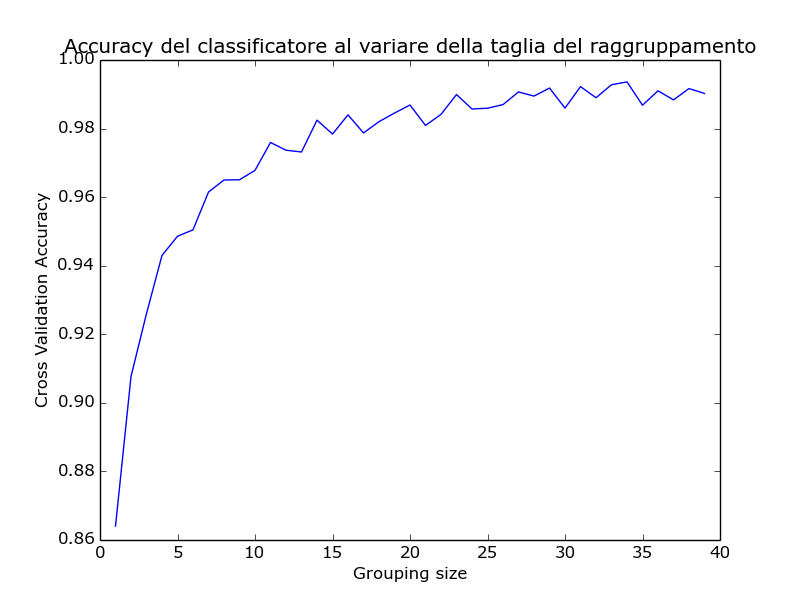
\includegraphics[width=\linewidth]{grouping.png}




\section{Spunti di ampliamento}

\nocite{*}
\printbibliography
\end{document}

